\documentclass[../main.tex]{subfiles}
\begin{document}

\chapter{Introduction}
\label{ch:introduction}


\section{Background}
\label{sec:background}


%\generalExpl{Present the background for the area. Set the context for your project – so that your reader can understand both your project and this thesis. (Give detailed background information in Chapter 2 - together with related work.)Sometimes it is useful to insert a system diagram here so that the reader knows what the different elements and their relationship to each other are. This also introduces the names/terms/… that you are going to use throughout your thesis (be consistent). This figure will also help you later delimit what you are going to do and what others have done or will do.}
Multiple \glsxtrfull{ML} techniques are based on the assumption of the manifold thesis \cite{fefferman_testing_2016}, which claims that high-dimensional data are samples from a lower dimensional manifold. There are multiple ways of utilizing this hypothesis, but we are going to focus on the Computational Topology perspective. \glsxtrfull{TDA} will give us the ability to answer the following questions about the qualitative geometric properties of our data sets: What are the topological features (such as connected components, number of holes, and number of cavities) of the underlying manifold? If we have introduced additional complexity to our data due to measurement or discretization problems, how do we measure the relevance of the observed features? 


Furthermore, as shown in \cite{hensel_survey_2021}, there is a rising interest in utilizing some of the techniques from TDA in \glsxtrfull{DL}. (a new field that could be named \glsxtrfull{TopoML}). In this survey, we can see that TDA tools are used in three distinct ways: incorporate the extraction of topological features as a layer in a \glsxtrfull{NN} (either as an input or a hidden layer), imposing certain properties based on the obtained topological information, and analyze the data and model architecture's topological properties to assess certain characteristics of the trained model.  

In this case, we are going to focus on the second option, i.e., see how we can impose certain properties by what we will call ``topological regularization''. Mainly we will develop the work proposed by Hofer \etal \cite{hofer_densified_2021}, where they prove that we can increase the generalization capabilities by imposing topological densification of each class distribution. Hence, the main idea is to condensate the density function of each class in the latent space so there is a better chance to have each class distribution contained in its decision region. The authors of the paper observed that we could impose that property by regularizing the size of the connected components using novel TopoML techniques.\\

One of the main fields that have studied the properties of latent spaces of ML models is Representation Learning. Furthermore, one of the main topics of interest in this field is to analyze the similarities of latent representation between networks. It has been shown in \cite{moschella_relative_2022} that by using ``relative latent representations,'' we can increase the similarities of latent spaces. The relative latent representation is obtained as follows: let $S\subset\mathcal{X}$ a dataset, $\varphi: \mathcal{X} \to \mathcal{Z}$ the feature extractor component of your network, and $\mathcal{A}=\{a_1, ..., a_k\}\subset\mathcal{X}$ a set of points called \emph{anchors}. Then for any similarity function $sim$ we define the relative representation of a point $x\in S$  w.r.t. $\mathcal{A}$ as
\[
(sim(\varphi(x), \varphi(a_1)), ..., sim(\varphi(x), \varphi(a_k))\in \mathbb{R}^k.
\]

Furthermore, the authors showcased that this technique allows zero-shot stitching, i.e., without additional fine-tuning, to be able to combine models with different architectures, datasets, or seeds, as shown in Figure \ref{fig:crossDomainScheme_intro}.\\

\begin{figure}[ht!]
     \centering
    \begin{subfigure}[b]{0.45\textwidth}
         \centering
         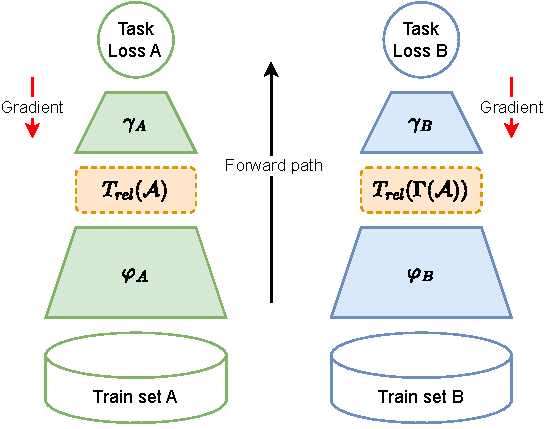
\includegraphics[width=\textwidth]{figures/bg/relativeTrainScheme.pdf}
        \caption{Train w/ relative transformations.}
         \label{fig:relTrainScheme_intro}
     \end{subfigure}\hfill
      \begin{subfigure}[b]{0.45\textwidth}
         \centering
         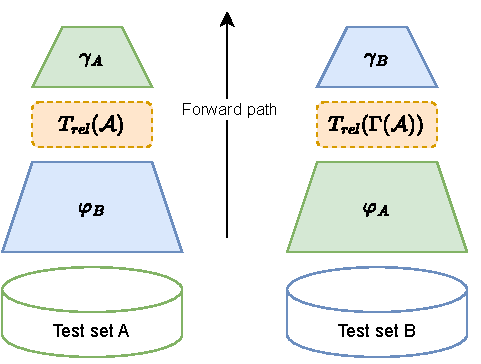
\includegraphics[width=0.9\textwidth]{figures/bg/relativeStitchScheme.pdf}
        \caption{Model stitching}
         \label{fig:relStitchScheme_intro}
     \end{subfigure}
    \caption{Cross-domain model stitching training and testing}
    \label{fig:crossDomainScheme_intro}
\end{figure}

Further details on the mathematical background and the described methods can be found in Chapter~\ref{ch:background}.

\section{Problem}
\label{sec:problem}


The main objective of this project is to try to expand the work proposed on \cite{hofer_densified_2021} into the setup proposed on \cite{moschella_relative_2022}, so we can have a better understanding of how these intrinsic representation regularization techniques interact with novel latent space representations.

% Research Question
\subsection{Research question}
\label{sec:researchQuestion}

Therefore our main research question is: To what extent does the application of the topological regularization method described in \cite{hofer_densified_2021} impact the classification performance of zero-shot stitching when utilizing relative latent representations \cite{moschella_relative_2022}?

\section{Purpose}
%\generalExpl{State the purpose  of your thesis and the purpose of your degree project. Describe who benefits and how they benefit if you achieve your goals. Include anticipated ethical, sustainability, social issues, etc. related to your project. (Return to these in your reflections in Section~\ref{sec:reflections}.)}

One of the purposes of this project is to showcase a brief introduction to TDA so that anyone with a ML background can comprehend the main philosophy and methodology proposed in this novel field of Topological Machine Learning. Furthermore, the work will be of interest to those interested in the fields of transfer learning and representation learning, who might want to know what will be the consequences of doing zero-shot stitching with models pretrained with topological regularization.\\

Also, the selected topological regularization is one of the few intrinsic representation regularization methods that has theoretically proven to increase generalization (instead of only using empirical evidence) \cite{hofer_densified_2021}. Therefore, this setup gives a lot of transparency to understand where could be the potential issues when combining the two methods.


\section{Goals}

%\generalExpl{State the goal/goals of this degree project.}
%\generalExpl{In addition to presenting the goal(s), you might also state what the deliverables and results of the project are.}


Since the selected topological regularization \cite{hofer_densified_2021} requires a supervised classification setup to be applied, then we will focus on studying the zero-shot stitching of encoders and decoders fine-tuned both with a relative representation. This deviates from the zero-shot setup presented in \cite{moschella_relative_2022} where only the decoder is finetuned with the relative representation (the encoder is frozen). Hence we have the following two main goals:

\begin{itemize}
    \item Analyse the performance of zero-shot stitching after fine-tuning the encoder and decoder with relative representation. Therefore our task would be to obtain a baseline for zero-shot of models trained with different datasets.
    
    \item Analyze the performance when training with the topological regularization and the relative representation. Which requires completing the following tasks:

    \begin{itemize}
         \item Analyse the functional and representational similarities of the latent spaces.
         
        \item Assess if the new representation is theoretically correct for the topological regularization.
        
        \item Assess the accuracy of the zero-shot stitching in this set-up.

        \item Assess whether we obtain better accuracy of the zero-shot stitching if we apply the topological regularization before or after the relative representation transformation.
        
    \end{itemize}
\end{itemize}

Lastly, an additional goal, we would want to know if our results depend on the specific construction to produce simplicial complexes in the TDA-based regularization. Therefore our tasks would be to analyze how we could  modify the arguments in \cite{hofer_densified_2021} with more accurate or efficient simplicial complex constructions. 


\section{Research Methodology}
%\generalExpl{Introduce your choice of methodology/methodologies and method/methods – and the reason why you chose them. Contrast them with and explain why you did not choose other methodologies or methods. (The details of the actual methodology and method you have chosen will be given in Chapter~\ref{ch:methods}. Note that in Chapter~\ref{ch:methods}, the focus could be research strategies, data collection, data analysis, and quality assurance.) In this section you should present your philosophical assumption(s), research method(s), and research approach(es).}

We are going to present a brief description of the methodology that we will pursue during this project in order to achieve the aforementioned goals. A more in-depth description of the methods can be seen in Chapter~\ref{ch:methods}.\\

First, we will compare the performance stated in \cite{hofer_densified_2021} to the one obtained when training while using relative representations (i.e., classification of basic CNN in CIFAR10 and MNIST). This will help us make a sanity check before assessing the tasks of the second objective.

Secondly, in order to assess the performance of the zero-shot stitching, we will try to replicate some of the experiments presented in \cite{moschella_relative_2022} adapted to our new setups. More specifically, we will compare the results of the Amazon review classification using cross-lingual stitching using a transformer language model fine-tuned (both encoder and decoder) with and without relative representations, as well as with and without topological regularization. 

Furthermore, we analyze the transferability between ViT models \cite{dosovitskiy_vit_2021} trained for the classification of lung and colon cancer histopathological images \cite{borkowski_lung_2019}. To have a more interesting setup, we will heavily reduce the part of the dataset corresponding to colon images. Hence, we will analyze the performance of zero-shot stitching combined with topological regularization in a more realistic scenario of image classification.\\

Thirdly, for the analysis of the characteristics, we could use some metrics such as the CKA \cite{kornblith_similarity_2019} in order to assess the similarity of the representations before and after the relative representation transformation.\\

Lastly, we have seen that some of the topological regularization techniques can be (potentially) improved when using some other simplicial complex structure (e.g., using Witness complexes \cite{schonenberger_witness_2022}). Hence, we will start checking if those structures can be applied in our case before looking for more specific structures.

\section{Delimitations}
%\generalExpl{Describe the boundary/limits of your thesis project and what you are explicitly not going to do. This will help you bound your efforts – as you have clearly defined what is out of the scope of this thesis project. Explain the delimitations. These are all the things that could affect the study if they were examined and included in the degree project.}

Our main goal will be to assess the impact of combining the previously defined methods (ablation studies) rather than analyze their performance under perfect conditions. Hence, based on this goal and acknowledging our time and computational constraints, we will not perform extensive hyperparameter tuning. 


Furthermore, in order to fulfill as many tasks as possible under our computational constraints, it might be necessary to use small datasets instead of big standard datasets such as Imagenet. Also, since we are working with ViT models, we might want to fine-tune a pretrained model (e.g., MAE \cite{he_masked_2021}) rather than training from scratch.

Lastly, we consider out of the scope of the project the study of zero-shot stitching under different architectures and different seeds.


\section{Structure of the thesis}\sweExpl{ Rapportens disposition}
Chapter~\ref{ch:background} presents relevant background information about xxx.  Chapter~\ref{ch:methods} presents the methodology and method used to solve the problem. …


\end{document}